% !TeX root = ../sameplaper.tex
% !TeX spellcheck = en_US

\chapter{Machine Learning Attacks}
\setcounter{section}{0}

\section{Machine Learning based Attack on LWE Problem}
Machine learning (ML) often assumes that given enough noisy data samples, it can learn the pattern from the samples. LWE problem, on the other hand, is based on the hardness assumption that states adding small noise to the inner product makes the secret recover hard. In general, the field of cryptanalysis and machine learning are closely related \cite{rivest1991cryptography}, both try to approximate the unknown function $F$ using the data at hand, however the context and techniques for doing so vary significantly between the fields.


Two key factors that make the LWE problem hard are the error and the use of modular arithmetic. Linear regression is enough to solve and find the secret in the absence of modular reduction; the use of modular reduction, on the other hand, requires performing linear regression on an $n$-dimensional torus, a much harder problem to solve. Recently, \cite{wenger2022salsa,li2023salsapic,li2023salsaver} looked into solving modular subset sum problems using transformers, which has been later mapped to solve the LWE problem.

Attacking LWE problem using machine learning (ML) is to find a model $M$ that learns to predict $y \in Y$ given $x \in X$. The model $M$ is usually computed via a supervised training process (model is trained with the (input, output) pairs). In the process, training values are processed to find a function that maps input values to an expected output value. The training process learns the the parameter $\theta$ of the model $M$ and are iteratively updated to minimize a predefined loss function $l(M,x,y,\Tilde{y})$, where $\Tilde{y}$ is the model's predicted output provided input $x$ and $y$ as its ground truth output.

In the LWE problem, the model is trained using LWE samples $(\textbf{a},b)$, putting it straight model is trained using input LWE samples $(\textbf{a},b)$ and asked to predict output $b$ for an unseen value of $\textbf{a}$, where $b=\textbf{a}\cdot\textbf{s}+\textbf{e}$. Here, for the loss function cross-entropy loss function - a well-known function in ML model training is used. For prediction, a well-known transformer architecture model is used, initially introduced for natural language processing (NLP) and machine translation. Transformers because of its accuracy and efficiency has been mapped to solve a wide range of problems, including text and image generation \cite{carion2020end}, image processing \cite{ramesh2021zero}, and speech recognition \cite{dong2018speech}. They are also adopted to solve problems in mathematics, like symbolic integration \cite{lample2019deep}, theorem proving \cite{polu2020generative}, and numerical computations \cite{charton2021linear}. Transformers are designed to process sequences of tokens; for example, in NLP, a sentence comprises of a sequences of words. Transformers usually combine a multi-head attention mechanism \cite{bahdanau2014neural} that takes care of relationship between different tokens in the sequence, essentially “decorrelating” it, and a fully connected neural network (FCNN), which processes the decorrelated sequences. A typical transformer used to solve the LWE problem in \cite{li2023salsa} is shown in the figure \ref{fig:transfromer_arch}.

\begin{figure}
    \centering
    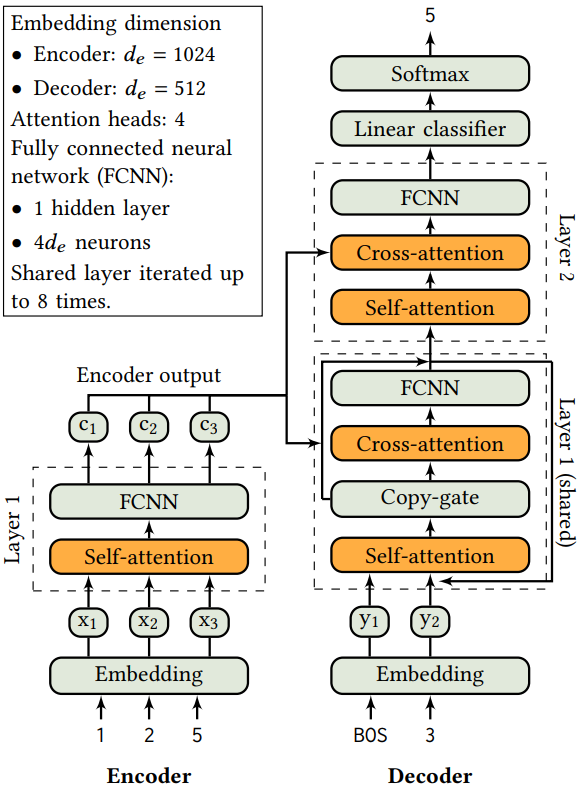
\includegraphics[width=.4\textwidth, height=.4\textwidth]{ML/Transformer_model.png}
    \caption{Transformer architecture used to solve the LWE problem taken from \cite{wenger2022salsa}}
    \label{fig:transfromer_arch}
\end{figure}

The overall attack methodology proceeds in three stages: data preprocessing, model training and  secret recovery as shown in the figure \ref{fig:attack_methodology}. The overall attack using ML proceeds as follows: Given $m$ LWE samples of fixed dimension $n$, modulus $q$ and with secret sampled from distribution $\chi$ the attack proceeds by performing following task in each of the above steps as follows.
\begin{figure}
    \centering
    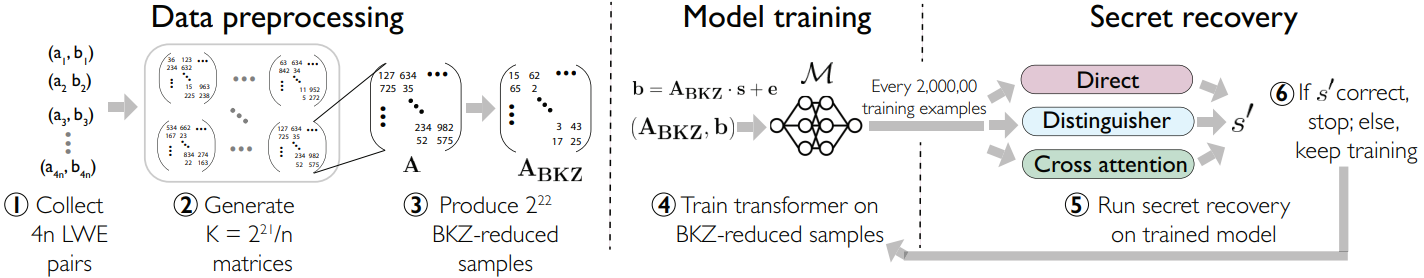
\includegraphics[width=\textwidth, height=.2\textwidth]{ML/Attack_methodology.png}
    \caption{Overall attack methodology using ML taken from \cite{li2023salsa}}
    \label{fig:attack_methodology}
\end{figure}

\paragraph{Data preprocessing}: In this step, $n$-LWE sample $(\textbf{a}_i,b_i)$ are subsampled from a pull of $m=4n$ samples to construct a matrix $\textbf{A}$ using $\textbf{a}_i$'s and to form a vector $\textbf{b}$ from $b_i$'s. Later, matrix $\textbf{A}$ is processed using some basis-reduction algorithm like LLL \cite{} or BKZ \cite{}; the same operations are performed on the vector $\textbf{b}$. The motivation behind the same is to obtain LWE samples with smaller coefficients to feed to the ML model, which performs better when the LWE sample entries are small.

This process is repeated to create $2^{21}/n$-matrices from ${4n \choose n}$ unique possible matrices. The subsampled $2^{21}/n$-matrices after reduction results in about $2^{22}$ (4 million) reduced LWE pairs. In general, the subsampled matrix contains duplicate rows, but after reduction, experimentally, no duplicate rows have been observed in the $4$ million created samples for dimension $n \geq 150$.

After sampling and recombination of LWE samples, lattice reduction is carried out on the lattice $\Lambda_i$ constructed using $n$ LWE samples $(\textbf{a},b)$ to make the LWE samples more amenable to the model training \cite{wenger2022salsa}. Subsample $n$-LWE sample to construct a lattice $\Lambda_i$ as shown below.
\begin{align*}
    \Lambda_i &= \begin{bmatrix}
                \omega \cdot \textbf{I}_n \hspace{1em} &  \textbf{A}_i  \\
                0                         \hspace{1em} &  q \cdot \textbf{I}_n
            \end{bmatrix}
\end{align*}
Here $n \times n$ matrix $\textbf{A}_i$ is constructed from $n$-LWE samples, $\textbf{I}_n$ is the identity matrix and $\omega \in \mathbb{Z}$ is the error penalization parameter.

Using lattice reduction algorithm BKZ to lattice $\Lambda_i$ transforms it by transformation $[\textbf{R}_i \hspace{1em} \textbf{C}_i]$, in such a way that the output matrix $[\omega \cdot \textbf{R} \hspace{1em}  \textbf{RA}+q\textbf{C}]$ will have $2n$ rows with small norms. Furthermore, the matrix $q\textbf{C}$ will add an integer multiple of $q$ to each entry in $\textbf{RA}$, so that all entries will be in the range $(-q/2,q/2)$.

\begin{align*}
    [\textbf{R}_{2n \times n} \hspace{1em} \textbf{C}_{2n \times n}]
    \begin{bmatrix}
        \omega \cdot \textbf{I}_n \hspace{1em} &  \textbf{A}_{n\times n} \\
        0                         \hspace{1em} &  q \cdot \textbf{I}_n
    \end{bmatrix} &=
    \begin{bmatrix}
        \omega \cdot \textbf{R}  \hspace{1em} &  \textbf{RA}+q\textbf{C}
    \end{bmatrix}
\end{align*}
Computed linear transformation $\textbf{R}$ is later applied to vector $\textbf{b}$ to create a new  LWE instance $(\textbf{RA},\textbf{Rb})$ with the same secret $\textbf{s}$ but reduced error $\textbf{e}'=\textbf{Rb}-\textbf{RA} \cdot \textbf{s}=\textbf{R}(\textbf{b}-\textbf{A}\cdot\textbf{s})=\textbf{Re}$ ($\textbf{e}=\textbf{b}-\textbf{A}\cdot \textbf{s}$). Thus, the final error depends on matrix $\textbf{R}$ values, and all values are computed under modulo $q$.

To control error amplification, parameter $\omega$ has been used. As stated earlier, BKZ computes $\textbf{R}$ and $\textbf{C}$ so that the norms of the row $[\omega \cdot \textbf{R} \hspace{1em}  \textbf{RA}+q\textbf{C}]$ are small. Large $\omega$ encourages small entries in the rows of $\textbf{R}$ but hinders the norm reduction of $\textbf{RA}+q\textbf{C}$ limiting the norm reduction of $\textbf{A}$ coordinates. In short, the choice of $\omega$ controls the trade-off between the reduction of $\textbf{a}$ we can achieve and the amount of additional noise injected in the transformed samples.

Recently, in \cite{li2023salsaver}, it has been observed that re-arranging the rows of lattice $\Lambda_i$ as
\begin{align*}
    \Lambda'_i &= \begin{bmatrix}
                0                         \hspace{1em} &  q \cdot \textbf{I}_n \\
                \omega \cdot \textbf{I}_n \hspace{1em} &  \textbf{A}_i
            \end{bmatrix}
\end{align*}
Results in a reduced number of operations needed for lattice reduction and allows BKZ to run with lower floating point precision. These two improvements cut the pre-processing time significantly.


\paragraph{Model training}: In this step the reduced LWE samples obtained from data preprocessing step above enters into the model training stage. For better understanding model training can be subdivided into following subcategories: data encoding, model architecture choice, and the training itself.

In data encoding step LWE samples are encoded in base $B$, as a sequence of tokens in $\{0, \cdots, B-1\}$. After encoding the coordinates of $\textbf{a}$ and $b$ are represented as two digit numbers in base $B$. Experiments performed for varying values of $B$ revels that large value of $B$, which limits the most significant digit of $a_i$ and $b$ to a small number of values provide better performance. Thus for all experiments value of $B$ is set to $B=\lfloor q/k \rfloor$ with $k=2\cdot \lceil \frac{n}{100}\rceil + 2$. However this creates a problem for large dimensions this is because large values of $q$ and $B$ results in large token vocabularies and is difficult to learn for the transformers with limited LWE samples. Mitigation of this is obtained by using encoding of the lowest digits of $\textbf{a}$ and $b$ into $B/r$ buckets of size $r$. Usually, $r$ is chosen in such a way that the  overall vocabulary size $B/r< 10,000$. Furthermore, usage of buckets helps training of models for large value of $n$ but have an impact on the loss of precision in the values of $\textbf{a}$ and $b$. However, it is believe that the impact on performance is limited, as it only affects the low bits of $\textbf{a}$ and $b$, which are anyways the most corrupted by LWE error.

The model architecture used for training and later to predict the value of $b$ is shown in figure \ref{fig:transfromer_arch}. The model, inspired from \cite{vaswani2017attention}, is a seq2seq model composed of two transformer stacks-- an encoder and a decoder, connected by a cross-attention mechanism. Here, the encoder gets the encoded discrete LWE samples as an input. The input sequence is first projected over a high-dimensional space (dimension $d=1024$ to be precise) by a Linear Embedding Layer with trainable weights (the embedding is learned during training, and initial embedding is generated using some seed). The resulting sequence is later processed by a single-layer transformer: a self-attention layer with four attention heads and a Fully connected neural network (FCNN) with one hidden layer of 4096 neurons.

The decoder is an auto-regressive model, which predicts the next token in the output sequence, given the already decoded output and the input sequence processed by the encoder. The decoder is provided a beginning of sequence token (BOS) and predicts $b_1^*$, the first digit of $b$. It is then fed the sequence BOS, $b_1^*$, and decoding proceeds until the end-of-sequence token (EOS) is output. The decoder input tokens are encoded as $512$-dimensional vectors via a trainable embedding. The decoder is made up of two layers. First, a shared layer, which is iterated through 8 times, feeds layer output back into its input. This recurrent process is controlled by a copy-gate mechanism, which decides whether a specific token should be processed by the shared layer or copied as is, skipping the next iteration. After eight iterations, the output of the shared layer is fed into a “regular” transformer layer. Finally, a linear layer processes the decoder output and computes the probability that any word in the vocabulary is the next token. The largest probability is selected via a softmax function.

As shown in the figure the decoder is connected to the encoder via a cross-attention mechanism with 4 attention heads. Speaking in more details, in each head, the output of the encoder $E=(E_i)_{i\in \mathbb{N}_l}$ ($l$ being the input sequence length) is multiplied by two trainable matrices, $W_k$ and $W_v$ , yielding the Keys $K$ = $W_k E$ and Values $V$ = $W_v E$. The 512-dimensional vector to be decoded, $D$, is multiplied by a matrix $W_Q$, yielding the Query $Q=W_Q D$. The $l$ scores are calculated from the query and keys as
\begin{align*}
    scores(E,D) = Softmax( (W_Q D) (W_K E)^T)
\end{align*}
The score calculated above measures the importance of each encoder input element when decoding $D$  i.e. while computing $b$. Usually, the cross-attention value for each head is the dot product of scores and values. Values of different heads are latter processed by a final linear layer. Cross-attention scores quantify the relation between input positions and output values. Picante uses them to recover the secret bit by bit.

The model $\textbf{M}$ discussed above is later used to predict $b$ from encoded $\textbf{a}$. The model $\textbf{M}$ treats it as a supervised multi-classification problem, by minimizing the loss function:

\begin{align*}
    min_{\theta \in \Theta} \sum_{i=1}^{N} \sum_{j=1}^{K} \sum_{k=1}^{V} \textbf{1}[y_i[j]=k-1] \frac{e^{\textbf{M}(x_i)[j,k]}} {\sum_{k'=1}^V e^{\textbf{M}(x_i)[j,k']}}
\end{align*}
The different parameters used in the model above are as follows: $\textbf{M}(x_i) \in \mathbb{R}^{K\times V}$ are the model logits evaluated at $x_i, \theta \in \Theta$, $N$ is the training sample size, $K=2$ is the output sequence length and $V=B/r$ is the vocabulary size.

To get prediction of $\textbf{M(a)}$ near to the ground truth $b$, the cross entropy needs to be minimized over all tokens in the output sequence. Bath traing is used to train the model with batch size $n_b=128$ examples. Furthermore, the cross-entropy loss $\textbf{L}(\textbf{M},\textbf{a},b)$ is computed over all batch examples and gradient $\nabla \textbf{L}$ are calculated with respect to the model parameters. Model parameters are later updated using the Adam optimized by $lr \nabla \textbf{L}$. $lr$ here represents the learning rate and is initially set to $10^{-5}$, except during the $1,000$ first optimizer steps, where it is increased linearly from $10^{-8}$ to $10^{-5}$. In the model used for computing the unknown secret, the model performance is evaluated after every epoch (epoch=$2$ million samples) on a held-out samples and secret recovery is tried if the it fails then another epoch begins.

%above are later encoded in base B and are used to train the model $M$. Training with sufficiently large number of LWE samples results in model $M$ being learned to predict $b$ from $\textbf{a}$. Usually, model training proceeds in epochs, each using 2 million samples. The 4 million training data are shuffled randomly every two epochs.

\paragraph{Secret recovery}: At the end of each epoch, the ML attack tries to recover the secret using different techniques. The intuition behind the same is that if the model $\textbf{M}$ can predict $b$ from $\textbf{a}$, then model $\textbf{M}$ somehow "knows" the secret $\textbf{s}$ and we can recover it from the model by enquiring the model. For secret recovery three techniques: direct, distinguisher, and cross-attention have been used. The different secret recovery techniques can be used standalone and can also be used in combination to recover the secret. Below we will discuss each techniques in more detail.

\paragraph{Direct secret recovery}: The idea behind this technique is to leverage the trained transformer's ability to generalize on inputs not seen during the training. To be precise, the training model is evaluated on special vector $\textbf{a}$ with one non-zero coordinate: $\textbf{a}=K\textbf{e}_i$ with $\textbf{e}_i$ the $i$-th standard basis vector and $K\in \mathbb{Z}_q$. For such vectors, since $b=\textbf{a}\cdot\textbf{s}+e$, and $\textbf{e}$ is small, $b\approx K$ if the $i$-th bit in the secret $\textbf{s}_i=1$and $b \approx 0$ otherwise. Usually, different $K_j$ are chosen, and the transformer is evaluated on $K_j\cdot e_i$ for $i=1,\cdots,n$, identifying potential $1$-bit in secret and producing a secret guess for each $K_j$.

\paragraph{Distinguisher secret recovery}: The general idea behind this technique is that if the $i$-th bit of the secret $s_i=0$ and $\textbf{e}_i$ is the $i$-th standard basis vector, then the model should predict close values for $\textbf{a}$ and $\textbf{a}+K .\textbf{e}_i$. Here the value of $b'=\textbf{M}(\textbf{a}+K \cdot \textbf{e}_i)$
is compared with $\textbf{M(a)}$. The rest remains the same; set the secret bits corresponding to the $h$ highest-scoring secret bits to $1$ and the rest to $0$.

\paragraph{Cross-Attention secret recovery}: This technique aims to recover the secret from the parameters of $\textbf{M}$ by leveraging the cross-attention scores of the first decoder layer. Intuitively, the cross-attention score measures the relevance of input tokens in the computation of $b$. Putting it simply, the coordinates of $\textbf{a}$ that correspond to the $0$ bits of $\textbf{s}$ have no impact on $b$, while the coordinates associated with the $1$ bits in $\textbf{s}$ have an impact proportional to their value in the calculation of $b$. Thus, we should get high-attention scores corresponding to the input positions $1$'s in the secret.


LWE problem is broadly categorized into three categories:
\begin{itemize}
    \item Easy: These are the category of LWE problem instances that are solvable via exhaustive search.
    \item Medium-to-hard: These category of LWE problem instances requires significant/unrealistic resources even for best known available attacks.
    \item Standardized: These category of LWE problem are the LWE problems that are believed secure or are not affordable to beak in a reasonable time using current computing facilities.
\end{itemize}

ML based attacks can break the Medium-to-hard LWE problems outperforming the lattice reduction attacks such as uSVP. However, it is still fur behind in breaking the LWE schemes standardized by NIST, which uses larger dimensions, smaller moduli $q$, and general secret distributions.
